\appendix

\chapter{Simulation Plots}

Here are listed additional plots generated from the simulations. The plots show the percentage change of isotopes in the simulation with different thorium concentrations. The plots show the percentage change in each step of simulation of each isotope. 

\begin{figure}[h]
    \centering
    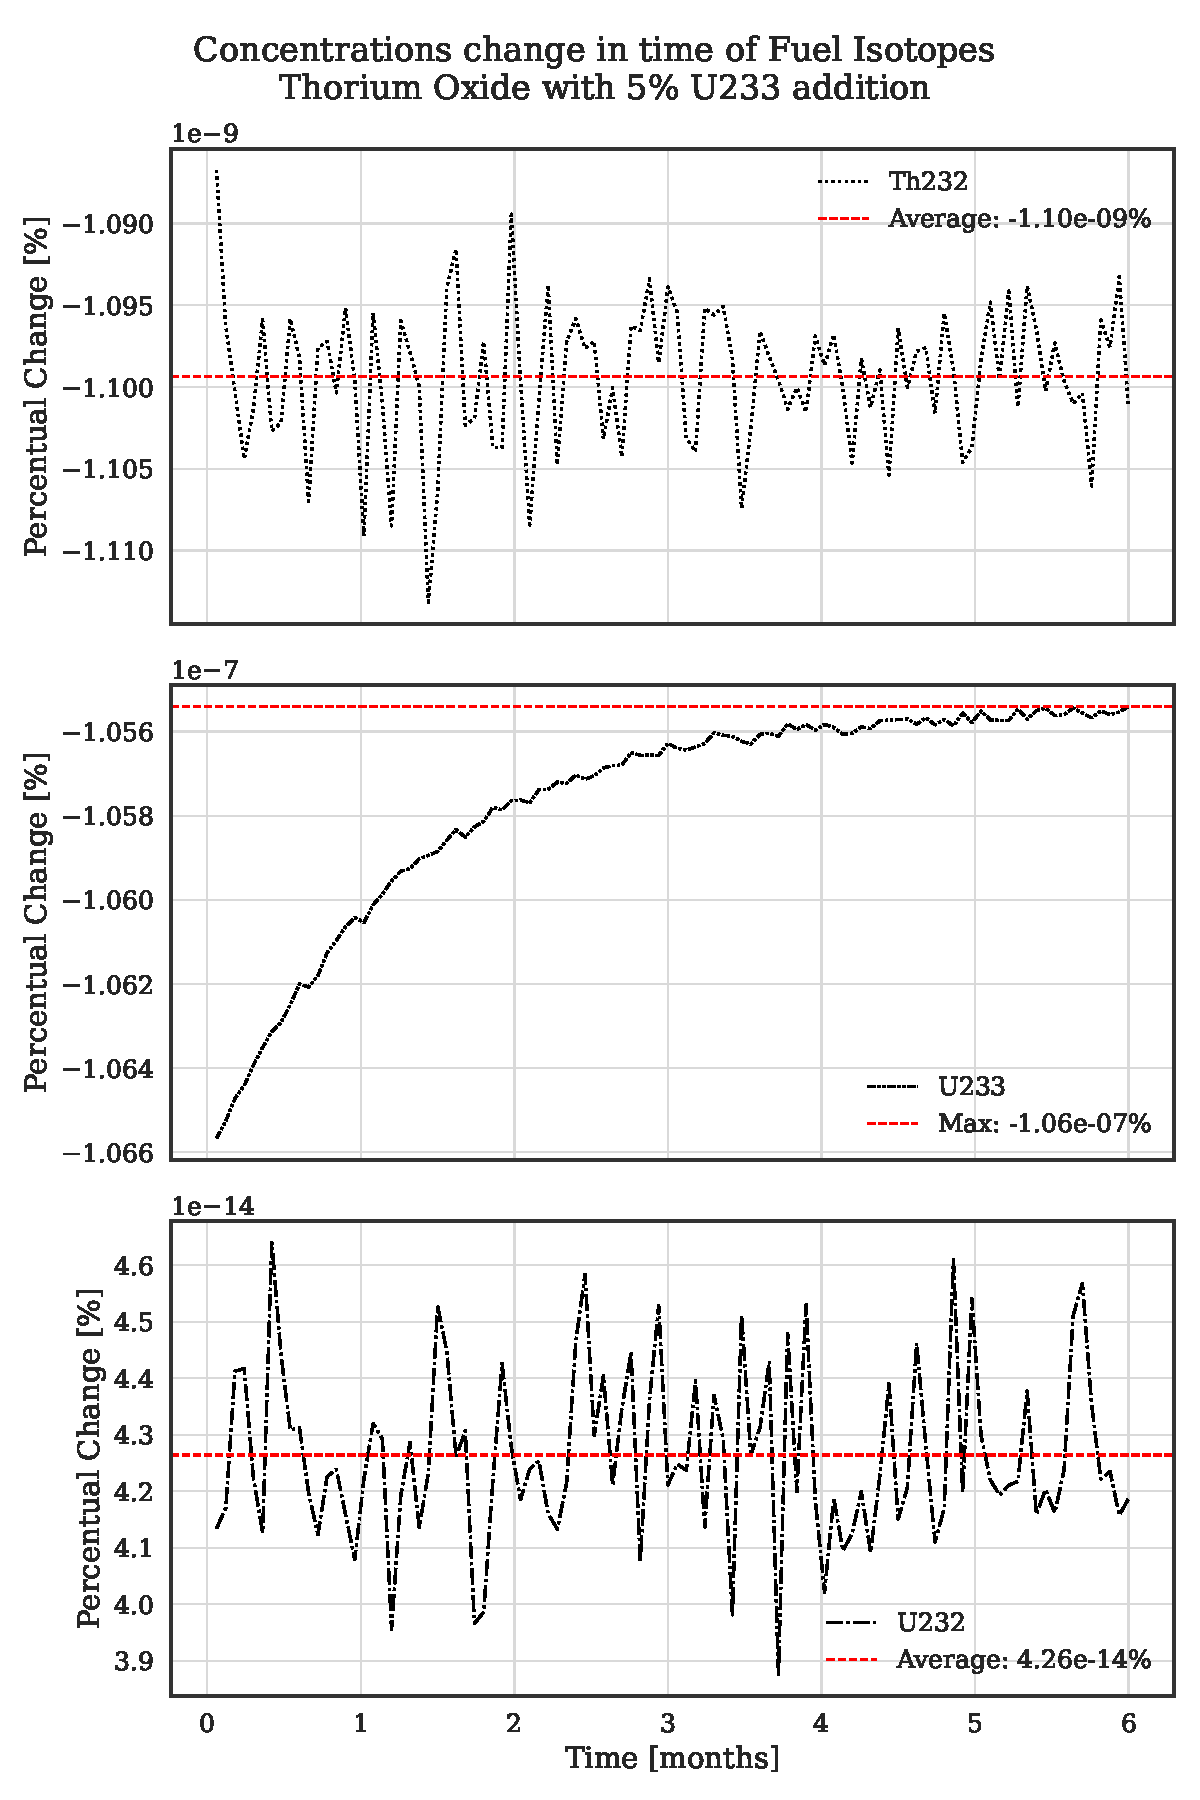
\includegraphics[width=0.75\textwidth, height=0.75\textheight]{Kap7/Figures_Kap7/percentual_change_th232_U233_5.pdf}
    \caption{Percentage change of isotopes in the simulation of a PWR fuel assembly using ThOX at \(5 \, \%\) \(\prescript{233}{}{U}\) concentration.}
    \label{fig:th_u233_5}
\end{figure}

\begin{figure}[h]
    \centering
    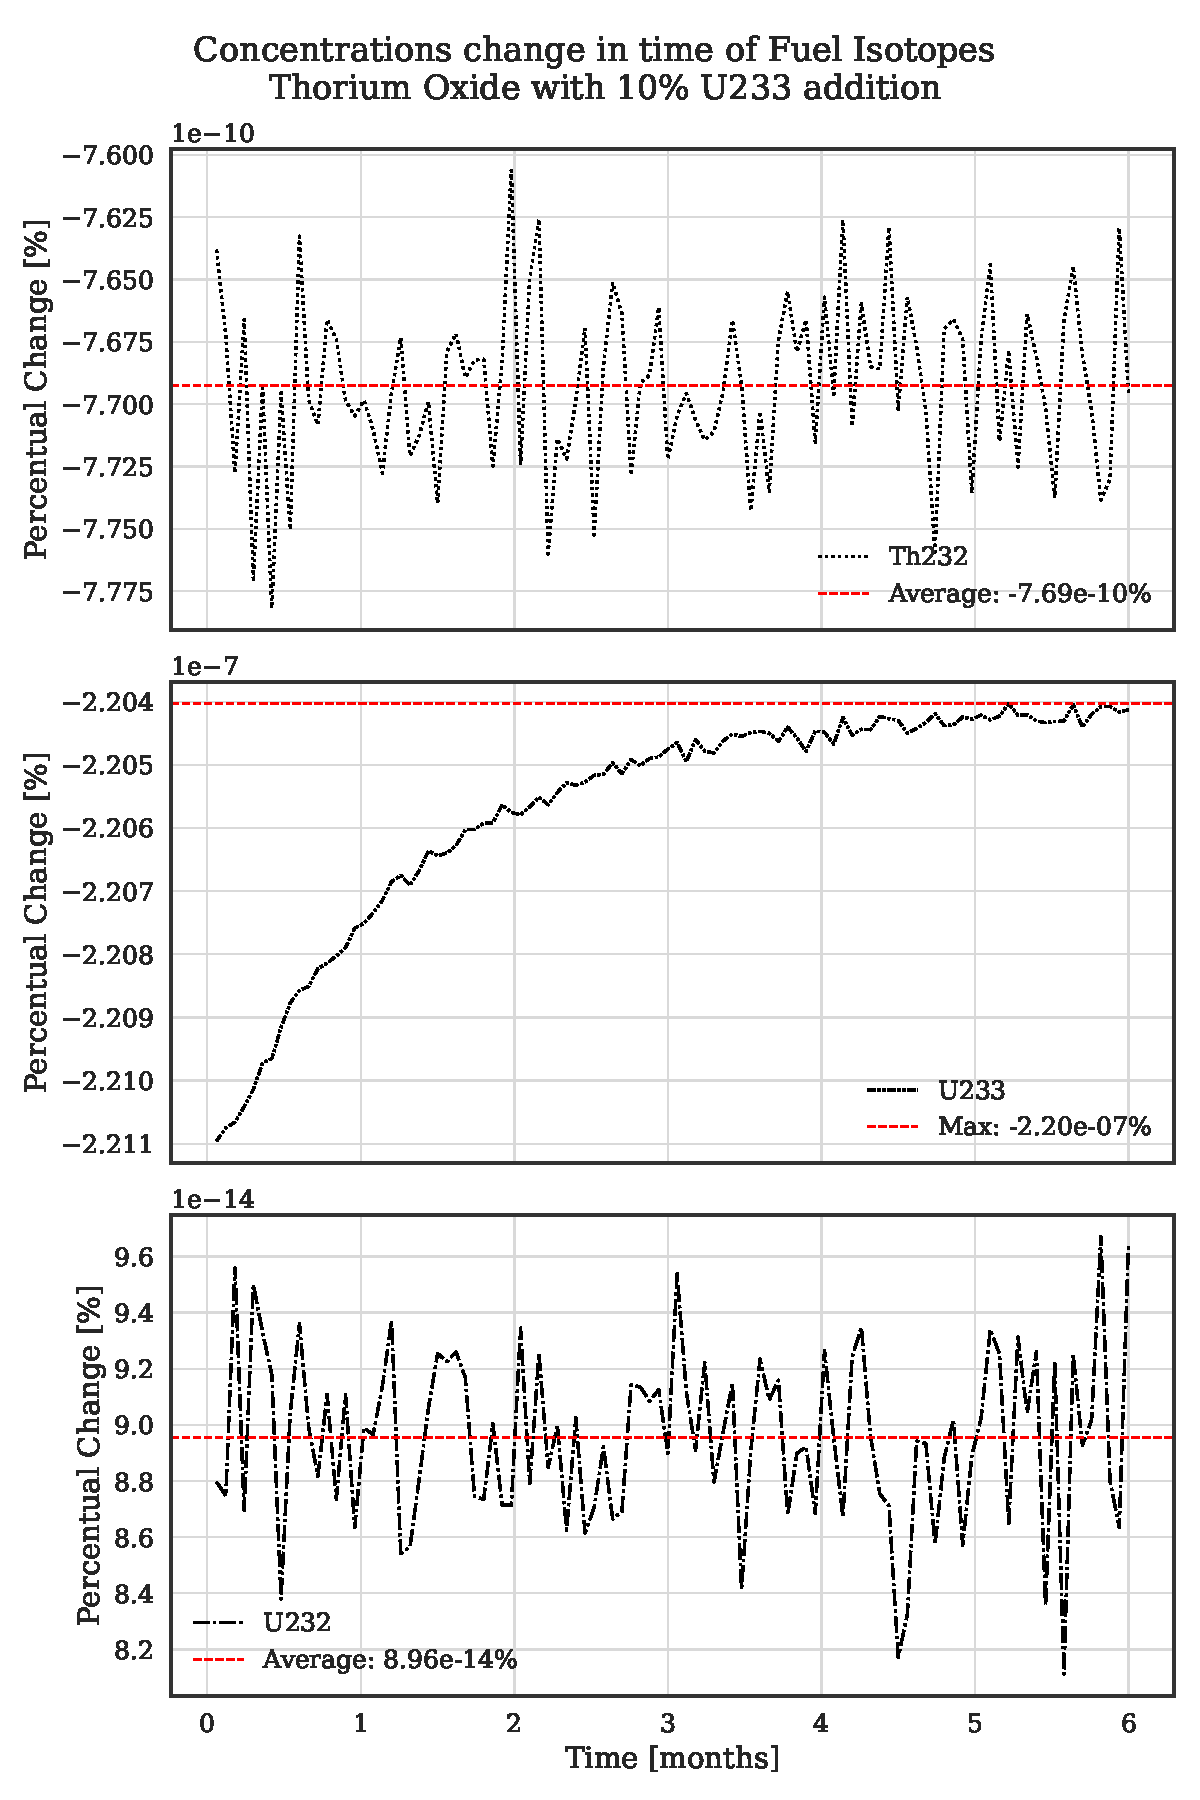
\includegraphics[width=0.75\textwidth, height=0.75\textheight]{Kap7/Figures_Kap7/percentual_change_th232_U233_10.pdf}
    \caption{Percentage change of isotopes in the simulation of a PWR fuel assembly using ThOX at \(10 \, \%\) \(\prescript{233}{}{U}\) concentration.}
    \label{fig:th_u233_10}
\end{figure}

\begin{figure}[h]
    \centering
    \includegraphics[width=1\textwidth]{Kap7/Figures_Kap7/percentual_change_uox.pdf}
    \caption{Percentage change of isotopes in the simulation of a PWR fuel assembly using UOX.}
    \label{fig:uo2}
\end{figure}

Finally, the following plots show the reactivity behavior of the fuel assemblies during the simulation. The reactivity is calculated as in \textbf{Eq} \ref{eq:def_reactivity}. It is noticeable that the reactivity of UOX, used as reference, is higher than \(0\) this is due to the consideration for the start of nuclear reactor, where it is needed this reactivity excess to ensure criticality of the reactor through the cycle.

\begin{figure}
    \centering
    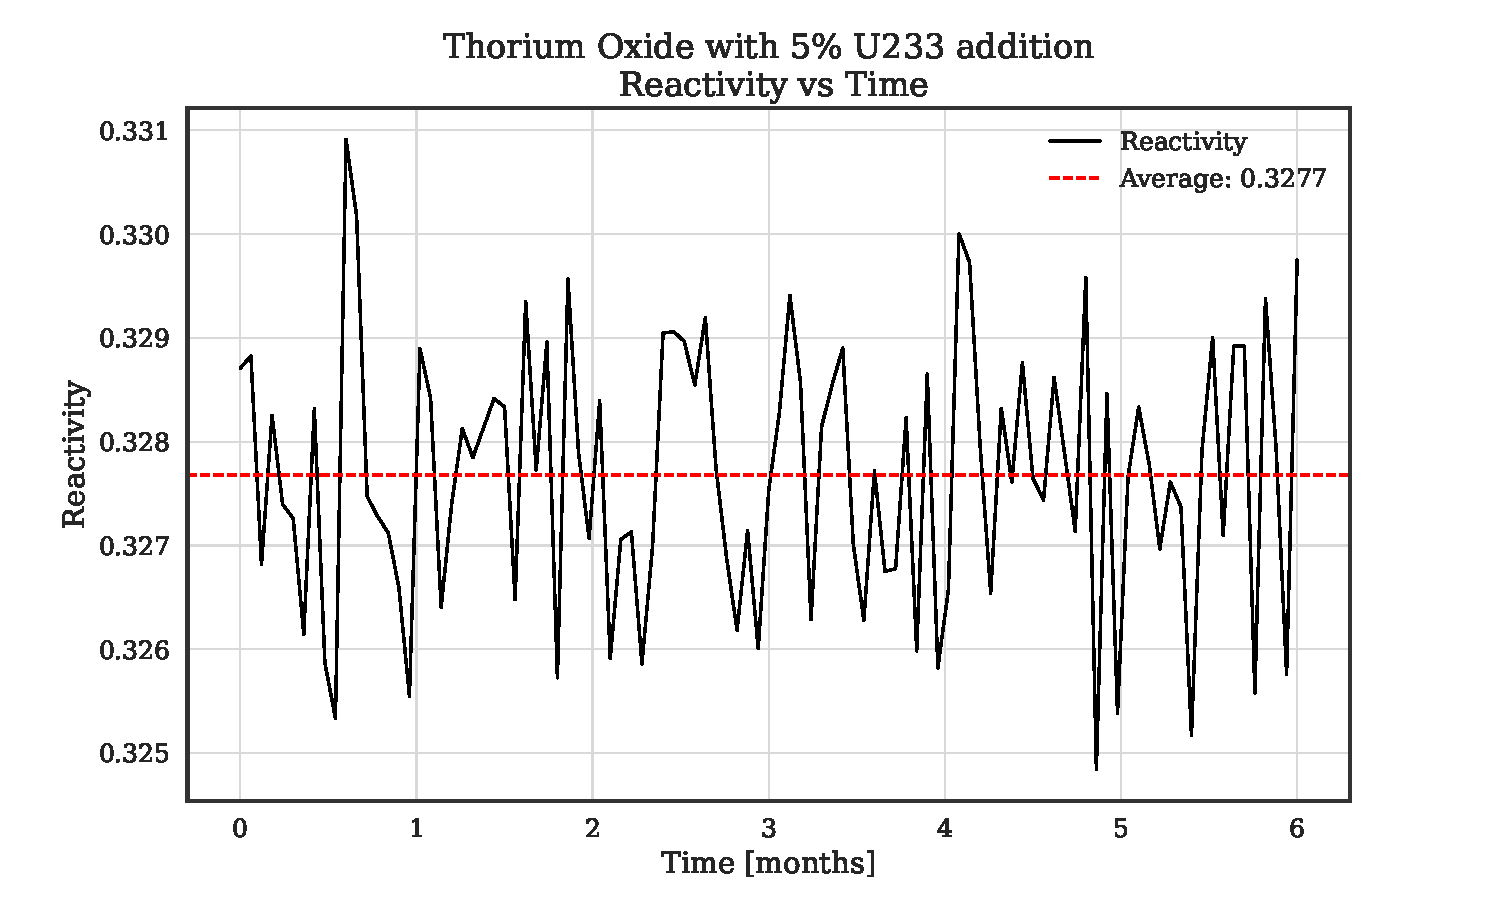
\includegraphics[width=1\textwidth, scale=0.5]{Kap7/Figures_Kap7/Reactivity_vs_Time_ThOX_U233_5.pdf}
    \caption{Reactivity of the simulation of a PWR fuel assembly using ThOX at \(5 \, \%\) \(\prescript{233}{}{U}\) concentration.}
    \label{fig:reactivity_th_u233_5}
\end{figure}

\begin{figure}
    \centering
    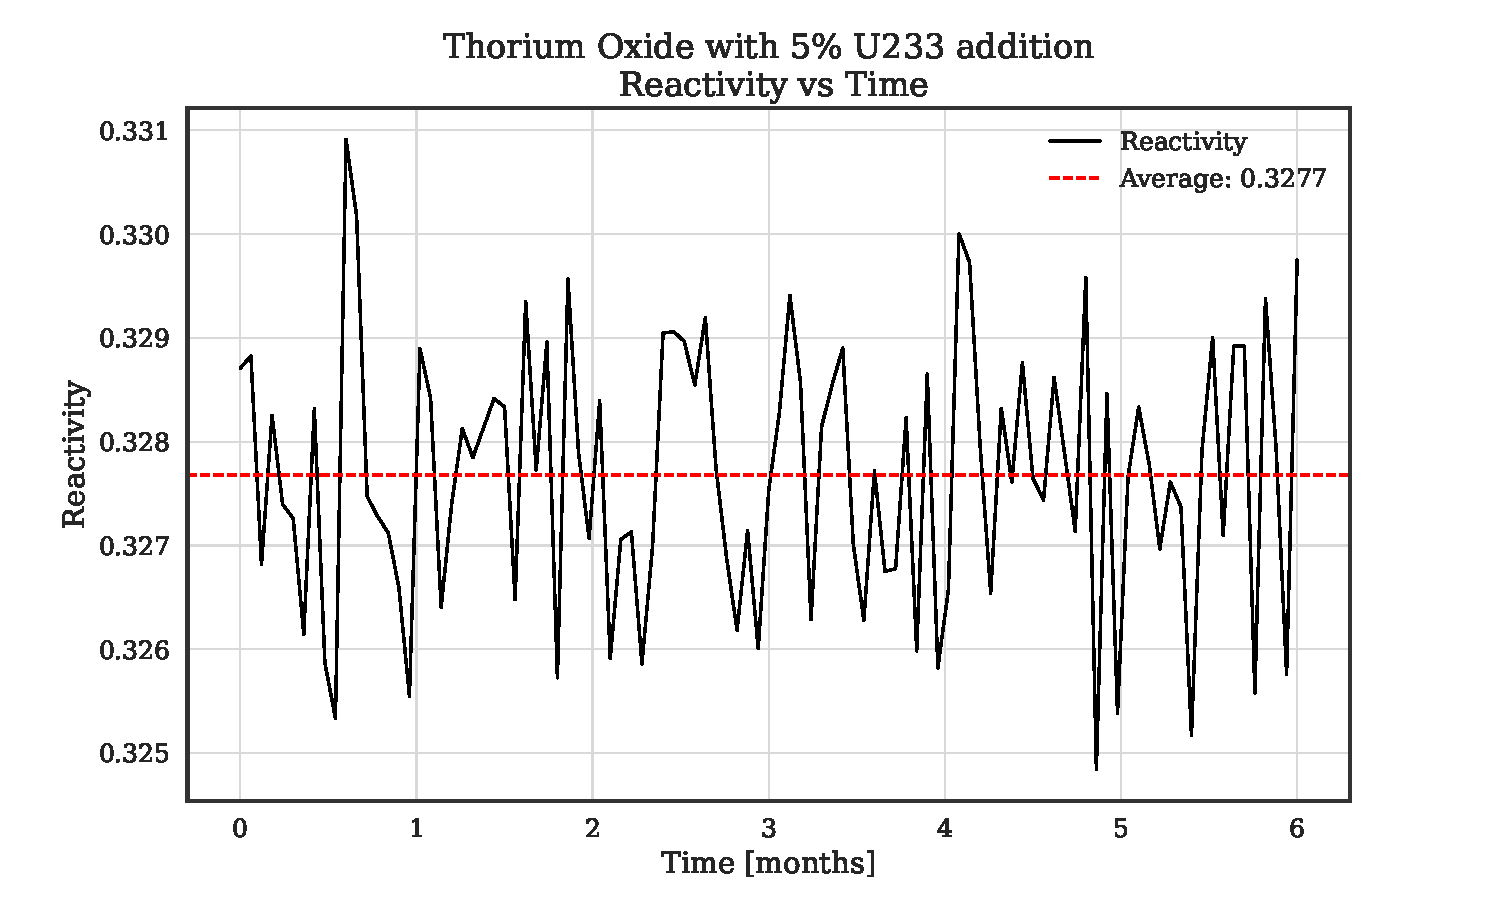
\includegraphics[width=1\textwidth, scale=0.5]{Kap7/Figures_Kap7/Reactivity_vs_Time_ThOX_U233_5.pdf}
    \caption{Reactivity of the simulation of a PWR fuel assembly using ThOX at \(10 \, \%\) \(\prescript{233}{}{U}\) concentration.}
    \label{fig:reactivity_th_u233_10}   
\end{figure}

\begin{figure}
    \centering
    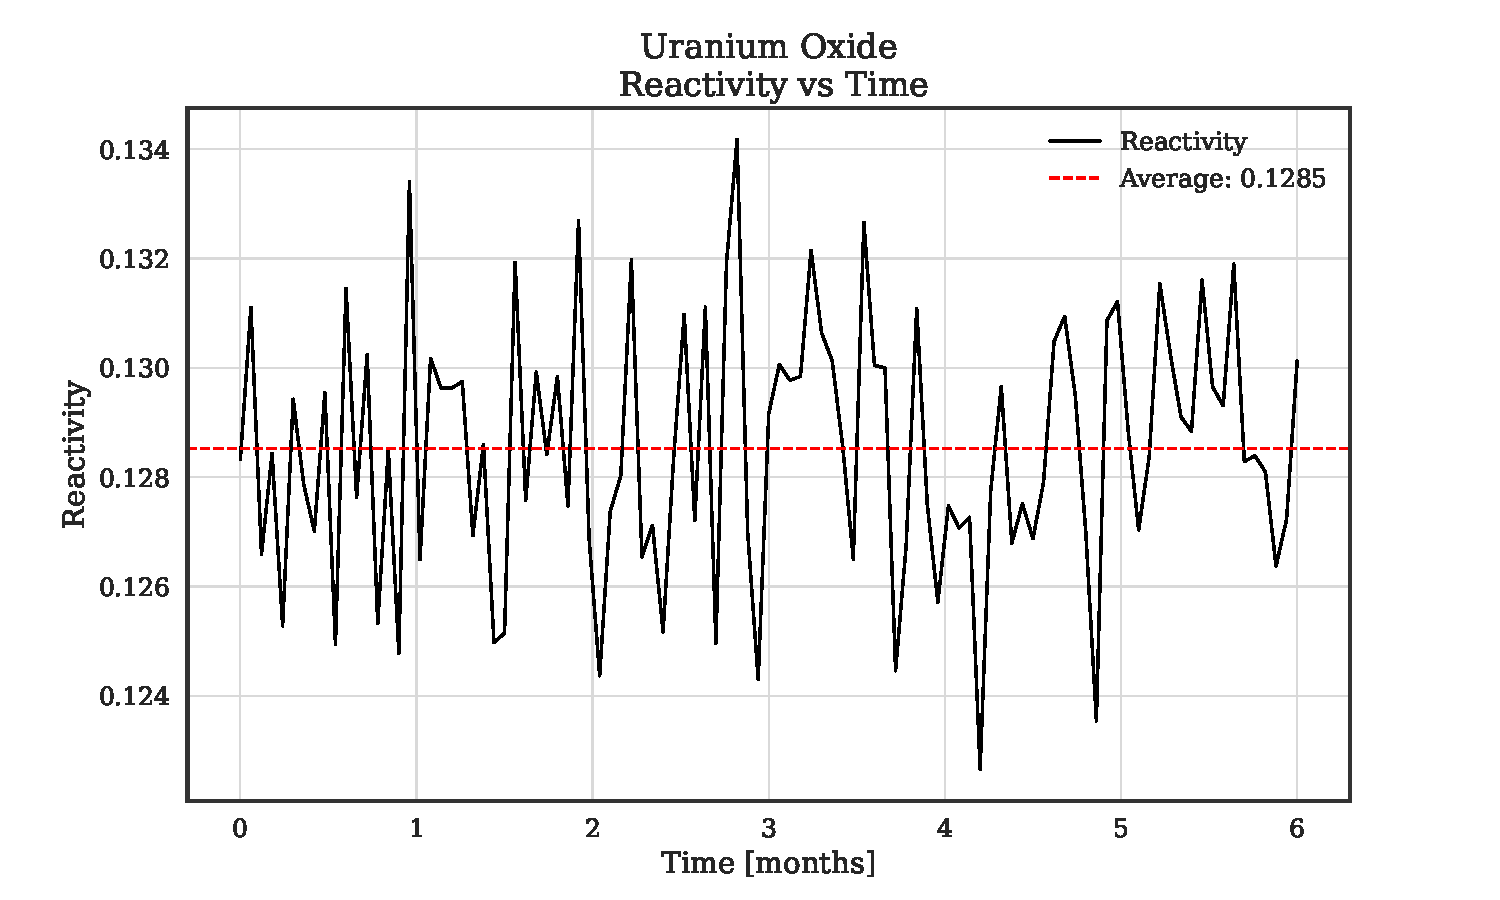
\includegraphics[width=1\textwidth, scale=0.5]{Kap7/Figures_Kap7/Reactivity_vs_Time_UOX.pdf}
    \caption{Reactivity of the simulation of a PWR fuel assembly using UOX.}
    \label{fig:reactivity_uox}
\end{figure}